\documentclass[border=4pt]{standalone}
\usepackage{amsmath,amssymb}
\usepackage{tikz}
\usetikzlibrary{arrows.meta,decorations.pathreplacing,calc,fit}
\definecolor{chA}{RGB}{31,94,170}
\definecolor{chB}{RGB}{200,90,20}
\definecolor{chC}{RGB}{30,130,80}
\begin{document}
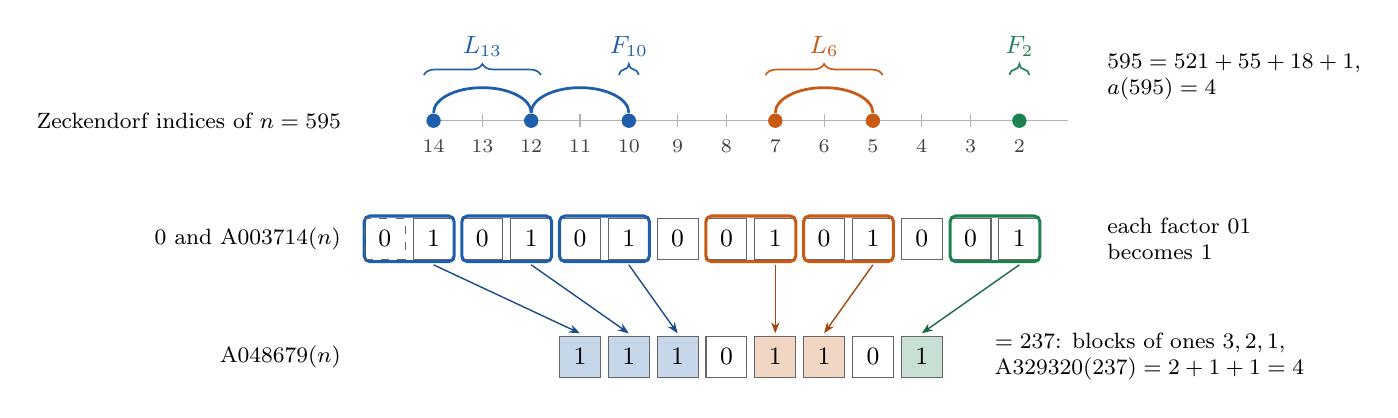
\begin{tikzpicture}[x=0.62cm,y=1cm,
  lab/.style={font=\small},
  note/.style={font=\footnotesize,align=left,anchor=west},
  bit/.style={draw=black!60,minimum size=5.2mm,inner sep=0pt,font=\small}]
  % row 1: Zeckendorf indices of n = 595 = F14+F12+F10+F7+F5+F2
  \node[note,anchor=east] at (-0.7,0) {Zeckendorf indices of $n=595$};
  \draw[gray!60] (1,0) -- (14,0);
  \foreach \k in {2,...,14} {
    \draw[gray!60] (15-\k,-0.08) -- (15-\k,0.08);
    \node[font=\scriptsize,gray!50!black] at (15-\k,-0.32) {$\k$};
  }
  \foreach \k/\col in {14/chA,12/chA,10/chA,7/chB,5/chB,2/chC} {
    \fill[\col] (15-\k,0) circle (2.6pt);
  }
  % chains: arcs of step 2
  \foreach \a/\b/\col in {14/12/chA,12/10/chA,7/5/chB} {
    \draw[\col,line width=1pt] (15-\a,0.1) arc[start angle=180,end angle=0,x radius=1,y radius=0.32];
  }
  % greedy merging
  \draw[decorate,decoration={brace,amplitude=4pt},line width=0.6pt,chA] (0.8,0.58) -- (3.2,0.58)
     node[midway,above=3pt,font=\small] {$L_{13}$};
  \draw[decorate,decoration={brace,amplitude=4pt},line width=0.6pt,chA] (4.8,0.58) -- (5.2,0.58)
     node[midway,above=3pt,font=\small] {$F_{10}$};
  \draw[decorate,decoration={brace,amplitude=4pt},line width=0.6pt,chB] (7.8,0.58) -- (10.2,0.58)
     node[midway,above=3pt,font=\small] {$L_{6}$};
  \draw[decorate,decoration={brace,amplitude=4pt},line width=0.6pt,chC] (12.8,0.58) -- (13.2,0.58)
     node[midway,above=3pt,font=\small] {$F_{2}$};
  \node[note] at (14.6,0.55) {$595=521+55+18+1$,\\ $a(595)=4$};
  % row 2: binary word of A003714(595), positions 12..0
  \node[note,anchor=east] at (-0.7,-1.5) {$0$ and $\mathrm{A003714}(n)$};
  \foreach \p/\b in {12/1,11/0,10/1,9/0,8/1,7/0,6/0,5/1,4/0,3/1,2/0,1/0,0/1} {
    \node[bit] (b\p) at (15-\p-2,-1.5) {$\b$};
  }
  % the factors 01 (preceded by 0) at positions k_i-1, k_i-2
  \foreach \p/\col in {13/chA,11/chA,9/chA,6/chB,4/chB,1/chC} {
    \draw[\col,line width=1.1pt,rounded corners=2pt] (15-\p-2-0.42,-1.79) rectangle (15-\p-2+1.42,-1.21);
  }
  \node[bit,dashed] at (0,-1.5) {$0$};
  \node[note] at (14.6,-1.5) {each factor $01$\\ becomes $1$};
  % row 3: A048679(595) = 11101101 = 237
  \node[note,anchor=east] at (-0.7,-3) {$\mathrm{A048679}(n)$};
  \foreach \i/\b/\col in {0/1/chA,1/1/chA,2/1/chA,3/0/white,4/1/chB,5/1/chB,6/0/white,7/1/chC} {
    \node[bit,fill=\col!25] at (2*\i/2+4,-3) {$\b$};
  }
  \foreach \from/\to/\col in {1/4/chA,3/5/chA,5/6/chA,8/8/chB,10/9/chB,13/11/chC} {
    \draw[-{Stealth[length=4pt]},\col!80!black,line width=0.5pt] (\from,-1.83) -- (\to,-2.7);
  }
  \node[note] at (12.3,-3) {$=237$: blocks of ones $3,2,1$,\\ $\mathrm{A329320}(237)=2+1+1=4$};
\end{tikzpicture}
\end{document}
